\documentclass{beamer}
\usepackage[utf8]{inputenc}

\usetheme{Copenhagen}
%color themes: default, beaver, beetle, seahorse, wolverine
\usecolortheme{default}
 
 
%Information to be included in the title page:
\title{Author Attribution of Turkish Texts by Feature Mining}
\author{Filiz Türkoğlu, Banu Diri, and M. Fatih Amasyalı} 
\institute{Narrators: Mehmetcan Güleşçi, Furkan Karakoyunlu}
\date{\today}
 
 
\begin{document}
 % Giriş sayfasını yazdır
 \frame{\titlepage}
 
 %scope slaytı
 \begin{frame}
  \frametitle{What is the problem?}
  \begin{itemize}
   \item One of the problems in text categorization is the authorship attribution, which is used to determine 
   the author of a text when it is not clear who wrote it
   \item In some occasions where two people claim to be the author of same manuscript 
   \item or on the contrary where no one is willing to accept the authorship of a document
  \end{itemize}
 \end{frame}
 
 \begin{frame}
  \frametitle{The aim of the article}
  \begin{itemize}
   \item They focused an author attribution of Turkish texts by extracting various feature vectors and applying 
   different classifiers
   \item They studied the comparative performance of classifier algorithms using the Naive Bayes, Support Vector 
   Machine, Random Forest, Multilayer Perceptron, and k-Nearest Neighbour
   \item To conclude they calculated the effectiveness of the methods by using 10-fold cross validation
  \end{itemize}
 \end{frame}

 \begin{frame}
  \frametitle{Early researches before this article}
  \begin{itemize}
   \item Early researchers in authorship attribution used a variety of statistical methods but it tends to vary 
   from author to author
   \begin{itemize}
    \item Mosteller and Wallace - Federalist Papers, by using set of function words
    \item Yule, by using complexity-based features (average sentence length, average word length, type/token 
    ratio ..)
    \item Recent technical advances in automated parsing and POS tagging, by using syntactic features such as 
    POS n-grams
    \item Peng, they modeled each author by a vector of the most frequent n-grams in the text
    \item Fung - Federalist Papers, by using Support Vector Machine classifier
    \item and so on (devamı çok uzun onları biz söyleriz 2 Authorship Attribution den önceki kısımda yazıyo 
    veya 1 slayt daha devam ederiz)
   \end{itemize}
  \end{itemize}
 \end{frame}
 
 \begin{frame}
  \frametitle{AUTHORSHIP ATTRIBUTION}
  \begin{itemize}
   \item In this article, they formed feature vectors from several categories of statistics
   \item Stylistic analysis in order to compare the efficacy of each
   \item They examined features in five main categories, which are statistical, vocabulary richness, grammatical, 
   lexical and n-grams model
   \item They obtained five different feature vectors from the mentioned categories
   \item Then, they created five feature subsets by using the feature selector to reduce the dimension of vectors
  \end{itemize}
 \end{frame}

 \begin{frame}
  \frametitle{Corpus}
  \begin{itemize}
   \item In this article, they used a corpus, 630 documents written by a single author are obtained from 35 texts per 
   18 different authors
   \item On different subjects like sport, popular interest and economics
   \item From Turkish daily newspaper, ``Hürriyet" and ''Vatan"
   \item In order to determine the authorship attribution performance in homogeneous and heterogeneous documents, 
   and different dataset sizes, this corpus is divided into 3 parts: Dataset I, Dataset II, Dataset III.
  \end{itemize}
 \end{frame}

 \begin{frame}
  \frametitle{General Feature Vector (gfv)}
  \begin{itemize}
   \item \textbf{Statistical features:} counting features in a text and applied this to word lengths and sentence lengths 
   \item \textbf{Vocabulary richness features:} there are different statistics to determine the richness of an author's vocabulary. 
   These features shows author's creativity.
   \item \textbf{Grammatical features:} based on Turkish Word Database (TWD) 35,000 words is used.
   \item \textbf{Function word features:} words that have little lexical meaning or have ambiguous meaning, 
   but instead serve to express grammatical relationships with order words within a sentence. 
  \end{itemize}
 \end{frame}
 
 \begin{frame}
  \frametitle{N-Gram Model}
  \begin{itemize}
   \item They extracted bi-grams and tri-grams
   \item While forming the bi-grams and the tri-grams of the corpus, they observed that the number of different bi-grams and 
   tri-grams are too much
   \item In order to avoid the combinatorial explosion in the feature vectors, they used a threshold value (greater than 75) 
   to reduce the number of features.
   \item After removed infrequent features, the dimensions of the bi-gram \textit{bgfv}, and tri-gram \textit{tgfv} feature vectors 
   are 470 and 1037 respectively.
   \item After that they combined \textit{bgfv} and \textit{tgfv}, they had a new feature vector(\textit{btgfv}) which has a dimension 
   of 1507.
   \item Finally they put together \textit{gfv} and \textit{btgfv} and obtained a 2148-dimensioned new vector, which is called 
   \textit{gbtgfv}.
  \end{itemize}
 \end{frame}
 
 \begin{frame}
  \frametitle{Feature Selection}
  \begin{itemize}
   \item A high number of features may slow down the process while giving similar results as obtained with much smaller feature subset.
   \item To learn the effect of high-dimensioned feature set over success ratio, they used CfsSubsetEval function which is in WEKA.
   \item They reduced features of general feature vector, \textit{gfv} and obtained a new vector, \textit{rgfv}.
   \begin{itemize}
    \item 24 dimension for Dataset I
    \item 17 dimension for Dataset II
    \item 40 dimension for Dataset III
   \end{itemize}
  \end{itemize}
 \end{frame}

  \begin{frame}
  \frametitle{Feature Selection}
  \begin{itemize}
   \item Same process was applied for Bi-gram feature vector, \textit{bgfv}, and was formed \textit{rbgfv}
   \begin{itemize}
    \item 25 features for Dataset I
    \item 20 features for Dataset II
    \item 63 features for Dataset III
   \end{itemize}
   \item They decreased dimension of Tri-gram feature vector, \textit{tgfv}, and obtained \textit{rtgfv}
   \begin{itemize}
    \item It has left 60 most distinguishing features for Dataset I
    \item 33 for Dataset II
    \item 101 for Dataset III
   \end{itemize}
   \item When features decreased from btgfv, rbtgfv is obtained. For Dataset I, vector has 61 features, for Dataset II it has 
   26 features, and for Dataset III it has 101 features.
  \end{itemize}
 \end{frame}
 
 \begin{frame}
  \frametitle{Feature Selection}
  \begin{itemize}
   \item They decreased dimension of \textit{gbtgfv}, and obtained \textit{rgbtgfv}. It has left 69 most distinguishing features for Dataset I, 30 for Dataset 
   II and 103 for Dataset III. All used feature vectors are shown at Table 1.
  \end{itemize}
  
  \begin{figure}[h]
    \begin{center}
      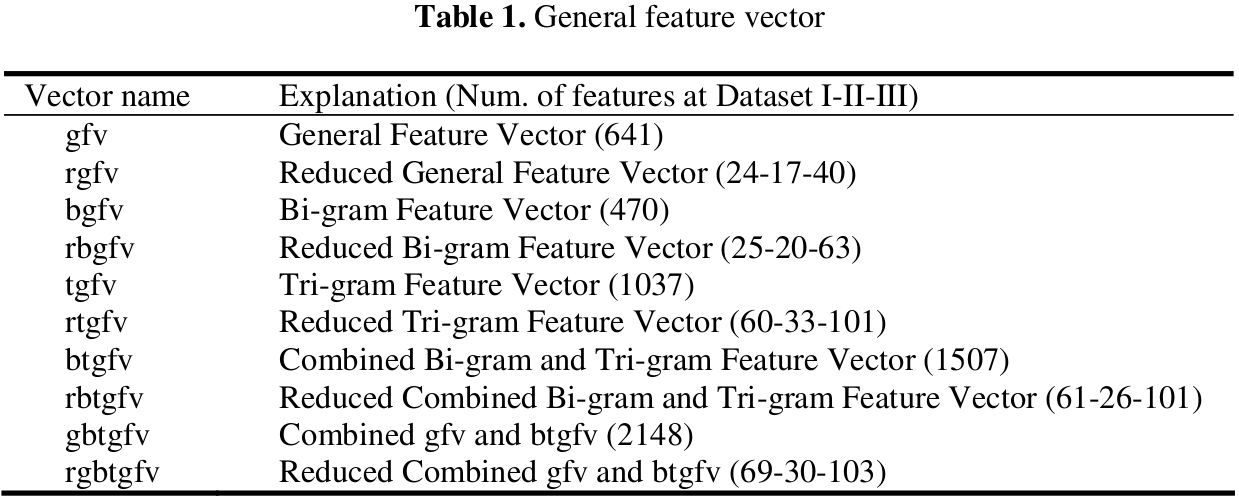
\includegraphics[scale=0.25]{table_1}
    \end{center}
   \end{figure}
 \end{frame}
 
 
 
\end{document}
